% Created by tikzDevice version 0.10.1 on 2016-04-29 09:31:53
% !TEX encoding = UTF-8 Unicode
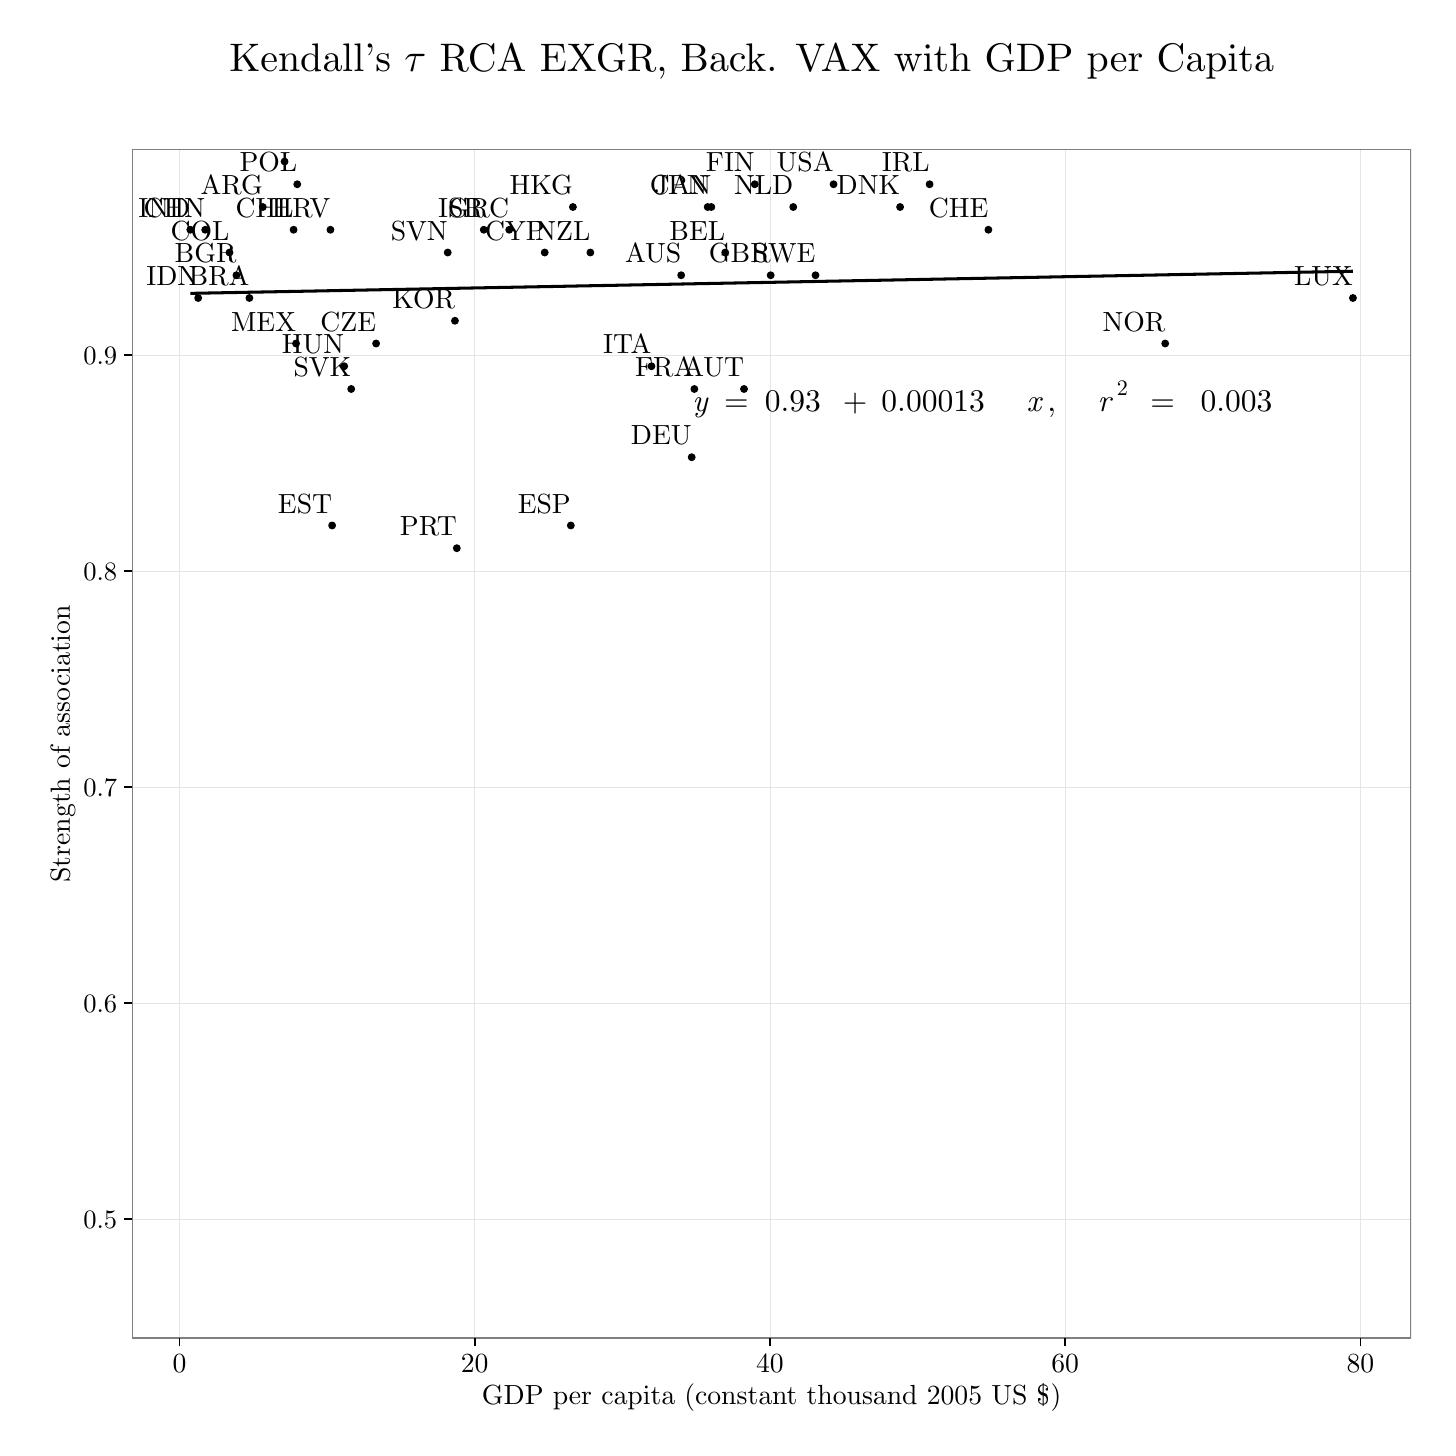
\begin{tikzpicture}[x=1pt,y=1pt]
\definecolor{fillColor}{RGB}{255,255,255}
\path[use as bounding box,fill=fillColor,fill opacity=0.00] (0,0) rectangle (505.89,505.89);
\begin{scope}
\path[clip] (  0.00,  0.00) rectangle (505.89,505.89);
\definecolor{drawColor}{RGB}{255,255,255}
\definecolor{fillColor}{RGB}{255,255,255}

\path[draw=drawColor,line width= 0.6pt,line join=round,line cap=round,fill=fillColor] (  0.00,  0.00) rectangle (505.89,505.89);
\end{scope}
\begin{scope}
\path[clip] ( 37.75, 32.37) rectangle (499.89,461.83);
\definecolor{fillColor}{RGB}{255,255,255}

\path[fill=fillColor] ( 37.75, 32.37) rectangle (499.89,461.83);
\definecolor{drawColor}{gray}{0.90}

\path[draw=drawColor,line width= 0.2pt,line join=round] ( 37.75, 75.32) --
	(499.89, 75.32);

\path[draw=drawColor,line width= 0.2pt,line join=round] ( 37.75,153.40) --
	(499.89,153.40);

\path[draw=drawColor,line width= 0.2pt,line join=round] ( 37.75,231.49) --
	(499.89,231.49);

\path[draw=drawColor,line width= 0.2pt,line join=round] ( 37.75,309.57) --
	(499.89,309.57);

\path[draw=drawColor,line width= 0.2pt,line join=round] ( 37.75,387.65) --
	(499.89,387.65);

\path[draw=drawColor,line width= 0.2pt,line join=round] ( 54.87, 32.37) --
	( 54.87,461.83);

\path[draw=drawColor,line width= 0.2pt,line join=round] (161.55, 32.37) --
	(161.55,461.83);

\path[draw=drawColor,line width= 0.2pt,line join=round] (268.23, 32.37) --
	(268.23,461.83);

\path[draw=drawColor,line width= 0.2pt,line join=round] (374.90, 32.37) --
	(374.90,461.83);

\path[draw=drawColor,line width= 0.2pt,line join=round] (481.58, 32.37) --
	(481.58,461.83);
\definecolor{drawColor}{RGB}{0,0,0}
\definecolor{fillColor}{RGB}{0,0,0}

\path[draw=drawColor,line width= 0.4pt,line join=round,line cap=round,fill=fillColor] ( 84.96,441.08)  circle (  1.21);

\path[draw=drawColor,line width= 0.4pt,line join=round,line cap=round,fill=fillColor] (236.13,416.42)  circle (  1.21);

\path[draw=drawColor,line width= 0.4pt,line join=round,line cap=round,fill=fillColor] (258.85,375.32)  circle (  1.21);

\path[draw=drawColor,line width= 0.4pt,line join=round,line cap=round,fill=fillColor] (252.05,424.64)  circle (  1.21);

\path[draw=drawColor,line width= 0.4pt,line join=round,line cap=round,fill=fillColor] ( 75.42,416.42)  circle (  1.21);

\path[draw=drawColor,line width= 0.4pt,line join=round,line cap=round,fill=fillColor] ( 80.12,408.20)  circle (  1.21);

\path[draw=drawColor,line width= 0.4pt,line join=round,line cap=round,fill=fillColor] (247.04,441.08)  circle (  1.21);

\path[draw=drawColor,line width= 0.4pt,line join=round,line cap=round,fill=fillColor] (347.15,432.86)  circle (  1.21);

\path[draw=drawColor,line width= 0.4pt,line join=round,line cap=round,fill=fillColor] ( 96.09,432.86)  circle (  1.21);

\path[draw=drawColor,line width= 0.4pt,line join=round,line cap=round,fill=fillColor] ( 64.15,432.86)  circle (  1.21);

\path[draw=drawColor,line width= 0.4pt,line join=round,line cap=round,fill=fillColor] ( 72.93,424.64)  circle (  1.21);

\path[draw=drawColor,line width= 0.4pt,line join=round,line cap=round,fill=fillColor] (186.82,424.64)  circle (  1.21);

\path[draw=drawColor,line width= 0.4pt,line join=round,line cap=round,fill=fillColor] (125.90,391.76)  circle (  1.21);

\path[draw=drawColor,line width= 0.4pt,line join=round,line cap=round,fill=fillColor] (239.94,350.67)  circle (  1.21);

\path[draw=drawColor,line width= 0.4pt,line join=round,line cap=round,fill=fillColor] (315.25,441.08)  circle (  1.21);

\path[draw=drawColor,line width= 0.4pt,line join=round,line cap=round,fill=fillColor] (196.27,326.01)  circle (  1.21);

\path[draw=drawColor,line width= 0.4pt,line join=round,line cap=round,fill=fillColor] (110.01,326.01)  circle (  1.21);

\path[draw=drawColor,line width= 0.4pt,line join=round,line cap=round,fill=fillColor] (262.73,449.30)  circle (  1.21);

\path[draw=drawColor,line width= 0.4pt,line join=round,line cap=round,fill=fillColor] (240.91,375.32)  circle (  1.21);

\path[draw=drawColor,line width= 0.4pt,line join=round,line cap=round,fill=fillColor] (268.48,416.42)  circle (  1.21);

\path[draw=drawColor,line width= 0.4pt,line join=round,line cap=round,fill=fillColor] (174.01,432.86)  circle (  1.21);

\path[draw=drawColor,line width= 0.4pt,line join=round,line cap=round,fill=fillColor] (197.02,441.08)  circle (  1.21);

\path[draw=drawColor,line width= 0.4pt,line join=round,line cap=round,fill=fillColor] (109.40,432.86)  circle (  1.21);

\path[draw=drawColor,line width= 0.4pt,line join=round,line cap=round,fill=fillColor] (114.37,383.54)  circle (  1.21);

\path[draw=drawColor,line width= 0.4pt,line join=round,line cap=round,fill=fillColor] ( 61.61,408.20)  circle (  1.21);

\path[draw=drawColor,line width= 0.4pt,line join=round,line cap=round,fill=fillColor] ( 58.76,432.86)  circle (  1.21);

\path[draw=drawColor,line width= 0.4pt,line join=round,line cap=round,fill=fillColor] (325.91,449.30)  circle (  1.21);

\path[draw=drawColor,line width= 0.4pt,line join=round,line cap=round,fill=fillColor] (164.81,432.86)  circle (  1.21);

\path[draw=drawColor,line width= 0.4pt,line join=round,line cap=round,fill=fillColor] (225.41,383.54)  circle (  1.21);

\path[draw=drawColor,line width= 0.4pt,line join=round,line cap=round,fill=fillColor] (245.72,441.08)  circle (  1.21);

\path[draw=drawColor,line width= 0.4pt,line join=round,line cap=round,fill=fillColor] (154.39,399.98)  circle (  1.21);

\path[draw=drawColor,line width= 0.4pt,line join=round,line cap=round,fill=fillColor] (478.88,408.20)  circle (  1.21);

\path[draw=drawColor,line width= 0.4pt,line join=round,line cap=round,fill=fillColor] ( 96.97,391.76)  circle (  1.21);

\path[draw=drawColor,line width= 0.4pt,line join=round,line cap=round,fill=fillColor] (276.64,441.08)  circle (  1.21);

\path[draw=drawColor,line width= 0.4pt,line join=round,line cap=round,fill=fillColor] (411.04,391.76)  circle (  1.21);

\path[draw=drawColor,line width= 0.4pt,line join=round,line cap=round,fill=fillColor] (203.33,424.64)  circle (  1.21);

\path[draw=drawColor,line width= 0.4pt,line join=round,line cap=round,fill=fillColor] ( 97.41,449.30)  circle (  1.21);

\path[draw=drawColor,line width= 0.4pt,line join=round,line cap=round,fill=fillColor] (155.07,317.79)  circle (  1.21);

\path[draw=drawColor,line width= 0.4pt,line join=round,line cap=round,fill=fillColor] (116.91,375.32)  circle (  1.21);

\path[draw=drawColor,line width= 0.4pt,line join=round,line cap=round,fill=fillColor] (151.78,424.64)  circle (  1.21);

\path[draw=drawColor,line width= 0.4pt,line join=round,line cap=round,fill=fillColor] (284.68,416.42)  circle (  1.21);

\path[draw=drawColor,line width= 0.4pt,line join=round,line cap=round,fill=fillColor] ( 92.83,457.52)  circle (  1.21);

\path[draw=drawColor,line width= 0.4pt,line join=round,line cap=round,fill=fillColor] (291.20,449.30)  circle (  1.21);

\node[text=drawColor,anchor=base east,inner sep=0pt, outer sep=0pt, scale=  1.0] at ( 84.96,445.52) {ARG};

\node[text=drawColor,anchor=base east,inner sep=0pt, outer sep=0pt, scale=  1.0] at (236.13,420.86) {AUS};

\node[text=drawColor,anchor=base east,inner sep=0pt, outer sep=0pt, scale=  1.0] at (258.85,379.77) {AUT};

\node[text=drawColor,anchor=base east,inner sep=0pt, outer sep=0pt, scale=  1.0] at (252.05,429.08) {BEL};

\node[text=drawColor,anchor=base east,inner sep=0pt, outer sep=0pt, scale=  1.0] at ( 75.42,420.86) {BGR};

\node[text=drawColor,anchor=base east,inner sep=0pt, outer sep=0pt, scale=  1.0] at ( 80.12,412.64) {BRA};

\node[text=drawColor,anchor=base east,inner sep=0pt, outer sep=0pt, scale=  1.0] at (247.04,445.52) {CAN};

\node[text=drawColor,anchor=base east,inner sep=0pt, outer sep=0pt, scale=  1.0] at (347.15,437.30) {CHE};

\node[text=drawColor,anchor=base east,inner sep=0pt, outer sep=0pt, scale=  1.0] at ( 96.09,437.30) {CHL};

\node[text=drawColor,anchor=base east,inner sep=0pt, outer sep=0pt, scale=  1.0] at ( 64.15,437.30) {CHN};

\node[text=drawColor,anchor=base east,inner sep=0pt, outer sep=0pt, scale=  1.0] at ( 72.93,429.08) {COL};

\node[text=drawColor,anchor=base east,inner sep=0pt, outer sep=0pt, scale=  1.0] at (186.82,429.08) {CYP};

\node[text=drawColor,anchor=base east,inner sep=0pt, outer sep=0pt, scale=  1.0] at (125.90,396.21) {CZE};

\node[text=drawColor,anchor=base east,inner sep=0pt, outer sep=0pt, scale=  1.0] at (239.94,355.11) {DEU};

\node[text=drawColor,anchor=base east,inner sep=0pt, outer sep=0pt, scale=  1.0] at (315.25,445.52) {DNK};

\node[text=drawColor,anchor=base east,inner sep=0pt, outer sep=0pt, scale=  1.0] at (196.27,330.45) {ESP};

\node[text=drawColor,anchor=base east,inner sep=0pt, outer sep=0pt, scale=  1.0] at (110.01,330.45) {EST};

\node[text=drawColor,anchor=base east,inner sep=0pt, outer sep=0pt, scale=  1.0] at (262.73,453.74) {FIN};

\node[text=drawColor,anchor=base east,inner sep=0pt, outer sep=0pt, scale=  1.0] at (240.91,379.77) {FRA};

\node[text=drawColor,anchor=base east,inner sep=0pt, outer sep=0pt, scale=  1.0] at (268.48,420.86) {GBR};

\node[text=drawColor,anchor=base east,inner sep=0pt, outer sep=0pt, scale=  1.0] at (174.01,437.30) {GRC};

\node[text=drawColor,anchor=base east,inner sep=0pt, outer sep=0pt, scale=  1.0] at (197.02,445.52) {HKG};

\node[text=drawColor,anchor=base east,inner sep=0pt, outer sep=0pt, scale=  1.0] at (109.40,437.30) {HRV};

\node[text=drawColor,anchor=base east,inner sep=0pt, outer sep=0pt, scale=  1.0] at (114.37,387.99) {HUN};

\node[text=drawColor,anchor=base east,inner sep=0pt, outer sep=0pt, scale=  1.0] at ( 61.61,412.64) {IDN};

\node[text=drawColor,anchor=base east,inner sep=0pt, outer sep=0pt, scale=  1.0] at ( 58.76,437.30) {IND};

\node[text=drawColor,anchor=base east,inner sep=0pt, outer sep=0pt, scale=  1.0] at (325.91,453.74) {IRL};

\node[text=drawColor,anchor=base east,inner sep=0pt, outer sep=0pt, scale=  1.0] at (164.81,437.30) {ISR};

\node[text=drawColor,anchor=base east,inner sep=0pt, outer sep=0pt, scale=  1.0] at (225.41,387.99) {ITA};

\node[text=drawColor,anchor=base east,inner sep=0pt, outer sep=0pt, scale=  1.0] at (245.72,445.52) {JPN};

\node[text=drawColor,anchor=base east,inner sep=0pt, outer sep=0pt, scale=  1.0] at (154.39,404.42) {KOR};

\node[text=drawColor,anchor=base east,inner sep=0pt, outer sep=0pt, scale=  1.0] at (478.88,412.64) {LUX};

\node[text=drawColor,anchor=base east,inner sep=0pt, outer sep=0pt, scale=  1.0] at ( 96.97,396.21) {MEX};

\node[text=drawColor,anchor=base east,inner sep=0pt, outer sep=0pt, scale=  1.0] at (276.64,445.52) {NLD};

\node[text=drawColor,anchor=base east,inner sep=0pt, outer sep=0pt, scale=  1.0] at (411.04,396.21) {NOR};

\node[text=drawColor,anchor=base east,inner sep=0pt, outer sep=0pt, scale=  1.0] at (203.33,429.08) {NZL};

\node[text=drawColor,anchor=base east,inner sep=0pt, outer sep=0pt, scale=  1.0] at ( 97.41,453.74) {POL};

\node[text=drawColor,anchor=base east,inner sep=0pt, outer sep=0pt, scale=  1.0] at (155.07,322.23) {PRT};

\node[text=drawColor,anchor=base east,inner sep=0pt, outer sep=0pt, scale=  1.0] at (116.91,379.77) {SVK};

\node[text=drawColor,anchor=base east,inner sep=0pt, outer sep=0pt, scale=  1.0] at (151.78,429.08) {SVN};

\node[text=drawColor,anchor=base east,inner sep=0pt, outer sep=0pt, scale=  1.0] at (284.68,420.86) {SWE};

\node[text=drawColor,anchor=base east,inner sep=0pt, outer sep=0pt, scale=  1.0] at ( 92.83,461.96) {TUR};

\node[text=drawColor,anchor=base east,inner sep=0pt, outer sep=0pt, scale=  1.0] at (291.20,453.74) {USA};

\path[draw=drawColor,line width= 1.1pt,line join=round] ( 58.76,409.87) --
	( 64.08,409.98) --
	( 69.39,410.08) --
	( 74.71,410.18) --
	( 80.03,410.28) --
	( 85.35,410.38) --
	( 90.67,410.48) --
	( 95.98,410.58) --
	(101.30,410.68) --
	(106.62,410.78) --
	(111.94,410.89) --
	(117.26,410.99) --
	(122.57,411.09) --
	(127.89,411.19) --
	(133.21,411.29) --
	(138.53,411.39) --
	(143.85,411.49) --
	(149.16,411.59) --
	(154.48,411.70) --
	(159.80,411.80) --
	(165.12,411.90) --
	(170.44,412.00) --
	(175.75,412.10) --
	(181.07,412.20) --
	(186.39,412.30) --
	(191.71,412.40) --
	(197.03,412.51) --
	(202.34,412.61) --
	(207.66,412.71) --
	(212.98,412.81) --
	(218.30,412.91) --
	(223.62,413.01) --
	(228.94,413.11) --
	(234.25,413.21) --
	(239.57,413.32) --
	(244.89,413.42) --
	(250.21,413.52) --
	(255.53,413.62) --
	(260.84,413.72) --
	(266.16,413.82) --
	(271.48,413.92) --
	(276.80,414.02) --
	(282.12,414.13) --
	(287.43,414.23) --
	(292.75,414.33) --
	(298.07,414.43) --
	(303.39,414.53) --
	(308.71,414.63) --
	(314.02,414.73) --
	(319.34,414.83) --
	(324.66,414.94) --
	(329.98,415.04) --
	(335.30,415.14) --
	(340.61,415.24) --
	(345.93,415.34) --
	(351.25,415.44) --
	(356.57,415.54) --
	(361.89,415.64) --
	(367.20,415.74) --
	(372.52,415.85) --
	(377.84,415.95) --
	(383.16,416.05) --
	(388.48,416.15) --
	(393.79,416.25) --
	(399.11,416.35) --
	(404.43,416.45) --
	(409.75,416.55) --
	(415.07,416.66) --
	(420.39,416.76) --
	(425.70,416.86) --
	(431.02,416.96) --
	(436.34,417.06) --
	(441.66,417.16) --
	(446.98,417.26) --
	(452.29,417.36) --
	(457.61,417.47) --
	(462.93,417.57) --
	(468.25,417.67) --
	(473.57,417.77) --
	(478.88,417.87);

\node[text=drawColor,anchor=base west,inner sep=0pt, outer sep=0pt, scale=  1.14] at (240.23,367.32) {\itshape y};

\node[text=drawColor,anchor=base west,inner sep=0pt, outer sep=0pt, scale=  1.14] at (251.68,367.32) {=};

\node[text=drawColor,anchor=base west,inner sep=0pt, outer sep=0pt, scale=  1.14] at (266.37,367.32) {0.93};

\node[text=drawColor,anchor=base west,inner sep=0pt, outer sep=0pt, scale=  1.14] at (294.56,367.32) {+};

\node[text=drawColor,anchor=base west,inner sep=0pt, outer sep=0pt, scale=  1.14] at (308.52,367.32) {0.00013};

\node[text=drawColor,anchor=base west,inner sep=0pt, outer sep=0pt, scale=  1.14] at (358.05,367.32) {};

\node[text=drawColor,anchor=base west,inner sep=0pt, outer sep=0pt, scale=  1.14] at (360.95,367.32) {\itshape x};

\node[text=drawColor,anchor=base west,inner sep=0pt, outer sep=0pt, scale=  1.14] at (368.47,367.32) {,};

\node[text=drawColor,anchor=base west,inner sep=0pt, outer sep=0pt, scale=  1.14] at (372.42,367.32) { };

\node[text=drawColor,anchor=base west,inner sep=0pt, outer sep=0pt, scale=  1.14] at (379.53,367.32) { };

\node[text=drawColor,anchor=base west,inner sep=0pt, outer sep=0pt, scale=  1.14] at (386.64,367.32) {\itshape r};

\node[text=drawColor,anchor=base west,inner sep=0pt, outer sep=0pt, scale=  0.8] at (393.56,373.14) {2};

\node[text=drawColor,anchor=base west,inner sep=0pt, outer sep=0pt, scale=  1.14] at (398.54,367.32) { };

\node[text=drawColor,anchor=base west,inner sep=0pt, outer sep=0pt, scale=  1.14] at (405.65,367.32) {=};

\node[text=drawColor,anchor=base west,inner sep=0pt, outer sep=0pt, scale=  1.14] at (416.72,367.32) { };

\node[text=drawColor,anchor=base west,inner sep=0pt, outer sep=0pt, scale=  1.14] at (423.83,367.32) {0.003};
\definecolor{drawColor}{gray}{0.50}

\path[draw=drawColor,line width= 0.6pt,line join=round,line cap=round] ( 37.75, 32.37) rectangle (499.89,461.83);
\end{scope}
\begin{scope}
\path[clip] (  0.00,  0.00) rectangle (505.89,505.89);
\definecolor{drawColor}{RGB}{0,0,0}

\node[text=drawColor,anchor=base east,inner sep=0pt, outer sep=0pt, scale=  0.96] at ( 32.35, 72.01) {0.5};

\node[text=drawColor,anchor=base east,inner sep=0pt, outer sep=0pt, scale=  0.96] at ( 32.35,150.10) {0.6};

\node[text=drawColor,anchor=base east,inner sep=0pt, outer sep=0pt, scale=  0.96] at ( 32.35,228.18) {0.7};

\node[text=drawColor,anchor=base east,inner sep=0pt, outer sep=0pt, scale=  0.96] at ( 32.35,306.26) {0.8};

\node[text=drawColor,anchor=base east,inner sep=0pt, outer sep=0pt, scale=  0.96] at ( 32.35,384.35) {0.9};
\end{scope}
\begin{scope}
\path[clip] (  0.00,  0.00) rectangle (505.89,505.89);
\definecolor{drawColor}{RGB}{0,0,0}

\path[draw=drawColor,line width= 0.6pt,line join=round] ( 34.75, 75.32) --
	( 37.75, 75.32);

\path[draw=drawColor,line width= 0.6pt,line join=round] ( 34.75,153.40) --
	( 37.75,153.40);

\path[draw=drawColor,line width= 0.6pt,line join=round] ( 34.75,231.49) --
	( 37.75,231.49);

\path[draw=drawColor,line width= 0.6pt,line join=round] ( 34.75,309.57) --
	( 37.75,309.57);

\path[draw=drawColor,line width= 0.6pt,line join=round] ( 34.75,387.65) --
	( 37.75,387.65);
\end{scope}
\begin{scope}
\path[clip] (  0.00,  0.00) rectangle (505.89,505.89);
\definecolor{drawColor}{RGB}{0,0,0}

\path[draw=drawColor,line width= 0.6pt,line join=round] ( 54.87, 29.37) --
	( 54.87, 32.37);

\path[draw=drawColor,line width= 0.6pt,line join=round] (161.55, 29.37) --
	(161.55, 32.37);

\path[draw=drawColor,line width= 0.6pt,line join=round] (268.23, 29.37) --
	(268.23, 32.37);

\path[draw=drawColor,line width= 0.6pt,line join=round] (374.90, 29.37) --
	(374.90, 32.37);

\path[draw=drawColor,line width= 0.6pt,line join=round] (481.58, 29.37) --
	(481.58, 32.37);
\end{scope}
\begin{scope}
\path[clip] (  0.00,  0.00) rectangle (505.89,505.89);
\definecolor{drawColor}{RGB}{0,0,0}

\node[text=drawColor,anchor=base,inner sep=0pt, outer sep=0pt, scale=  1.00] at ( 54.87, 20.09) {0};

\node[text=drawColor,anchor=base,inner sep=0pt, outer sep=0pt, scale=  1.00] at (161.55, 20.09) {20};

\node[text=drawColor,anchor=base,inner sep=0pt, outer sep=0pt, scale=  1.00] at (268.23, 20.09) {40};

\node[text=drawColor,anchor=base,inner sep=0pt, outer sep=0pt, scale=  1.00] at (374.90, 20.09) {60};

\node[text=drawColor,anchor=base,inner sep=0pt, outer sep=0pt, scale=  1.00] at (481.58, 20.09) {80};
\end{scope}
\begin{scope}
\path[clip] (  0.00,  0.00) rectangle (505.89,505.89);
\definecolor{drawColor}{RGB}{0,0,0}

\node[text=drawColor,anchor=base,inner sep=0pt, outer sep=0pt, scale=  1.00] at (268.82,  8.40) {GDP per capita (constant thousand 2005 US \$)};
\end{scope}
\begin{scope}
\path[clip] (  0.00,  0.00) rectangle (505.89,505.89);
\definecolor{drawColor}{RGB}{0,0,0}

\node[text=drawColor,rotate= 90.00,anchor=base,inner sep=0pt, outer sep=0pt, scale=  1.00] at ( 15.29,247.10) {Strength of association};
\end{scope}
\begin{scope}
\path[clip] (  0.00,  0.00) rectangle (505.89,505.89);
\definecolor{drawColor}{RGB}{0,0,0}

\node[text=drawColor,anchor=base west,inner sep=0pt, outer sep=0pt, scale=  1.44] at ( 72.87,489.97) {Kendall's $\tau$ RCA EXGR, Back. VAX with GDP per Capita};
\end{scope}
\end{tikzpicture}
